\documentclass[a4paper,english]{article}

\usepackage[dvips]{graphicx}
\usepackage[top=2cm,bottom=3cm,left=2cm,right=1cm]{geometry}
\usepackage{amsmath}
\usepackage{subfigure}

\title{Machine Intelligence 2 \\ Exercise sheet 7}
\author{Group 1 \\Tiziano, Raphael, Stephan}
\date{\today}
\begin{document}
\maketitle


\section*{Exercise 1 - Kurtosis of Toy Data}

In this exercise we can have a feeling about the meaning of kurtosis. Rotating randomly distributed data (after spheering) we can achieve different values of kurtosis for different dimensions.
Since we de-corellate the data, samples are distributed along orthogonal directions; this results in a phase shift of $\pi$ when the kurtosis is estimated for the two dimensions as a function of the rotation angle. From these plots we can see that the kurtosis is a measure of how ``peaky'' is a distribution compared to a gaussian. This is particularly clear in the example with the uniform distribution.

\begin{figure}
\centering
\subfigure[original]{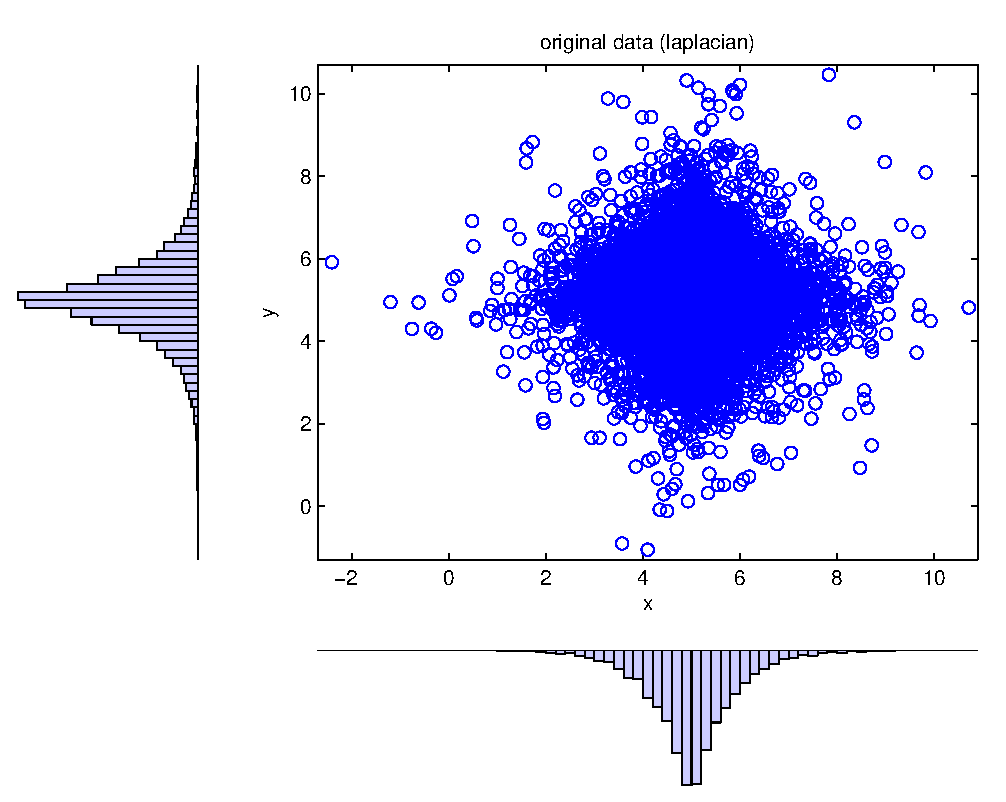
\includegraphics[scale = .4]{laplacian_original.eps}}\qquad
\subfigure[mixed]{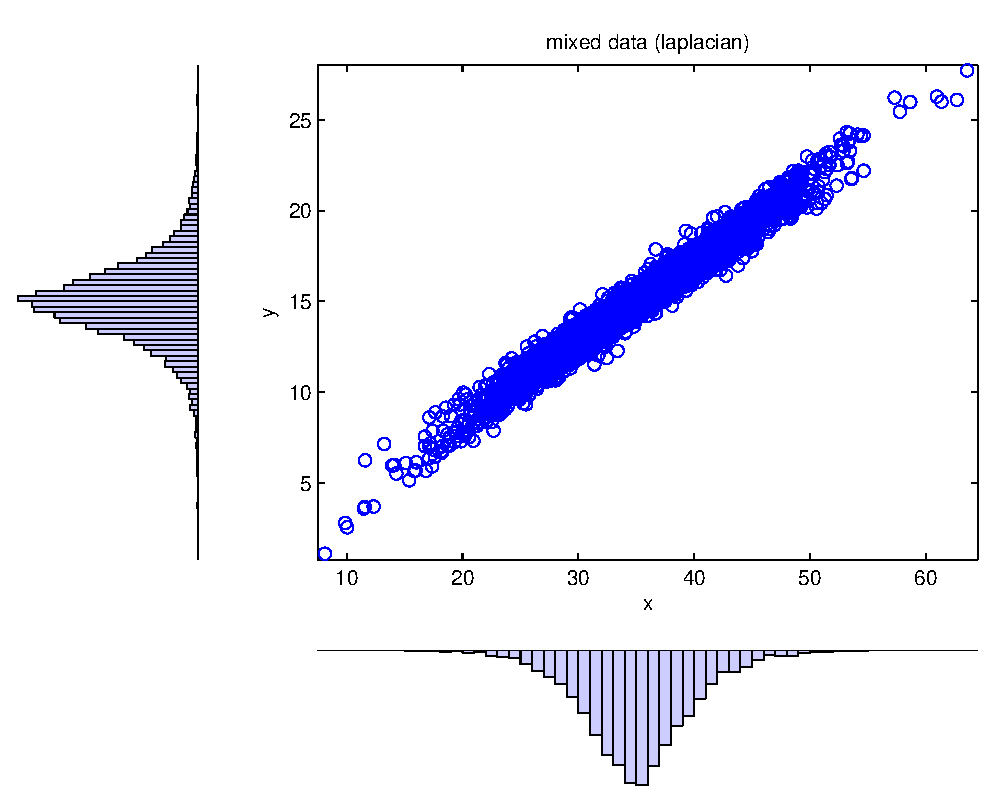
\includegraphics[scale = .4]{laplacian_mixed.eps}} \\
\subfigure[centered]{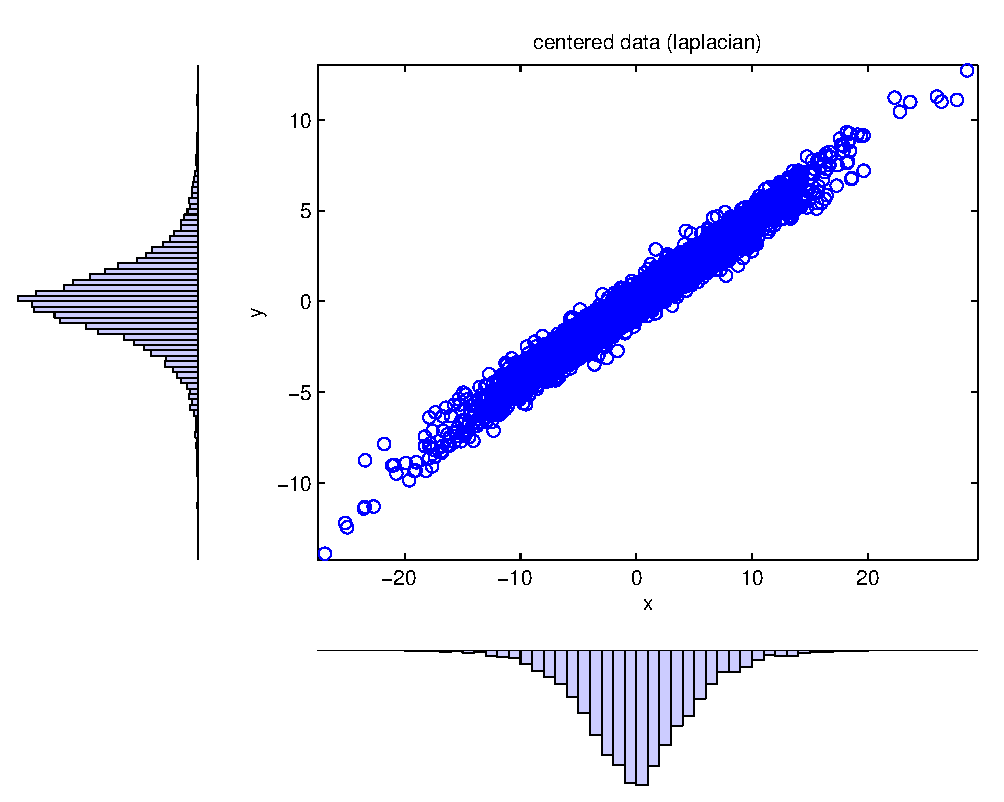
\includegraphics[scale = .4]{laplacian_centered.eps}}\qquad
\subfigure[decorellated]{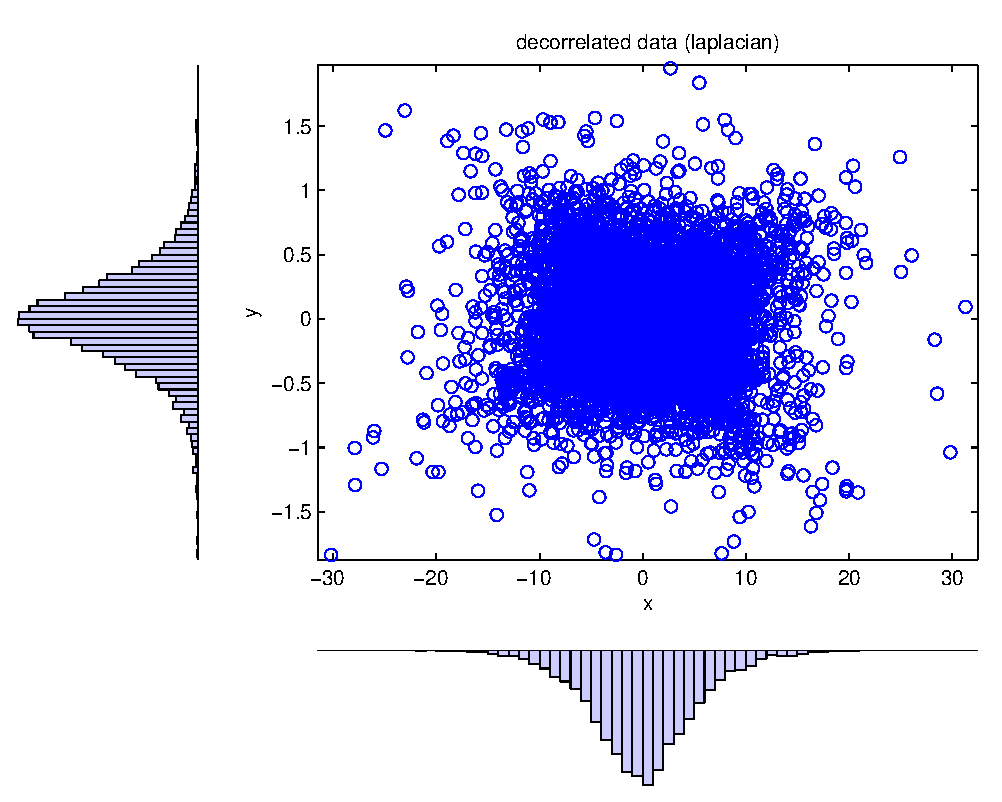
\includegraphics[scale = .4]{laplacian_decorellated.eps}} \\
\subfigure[spheered]{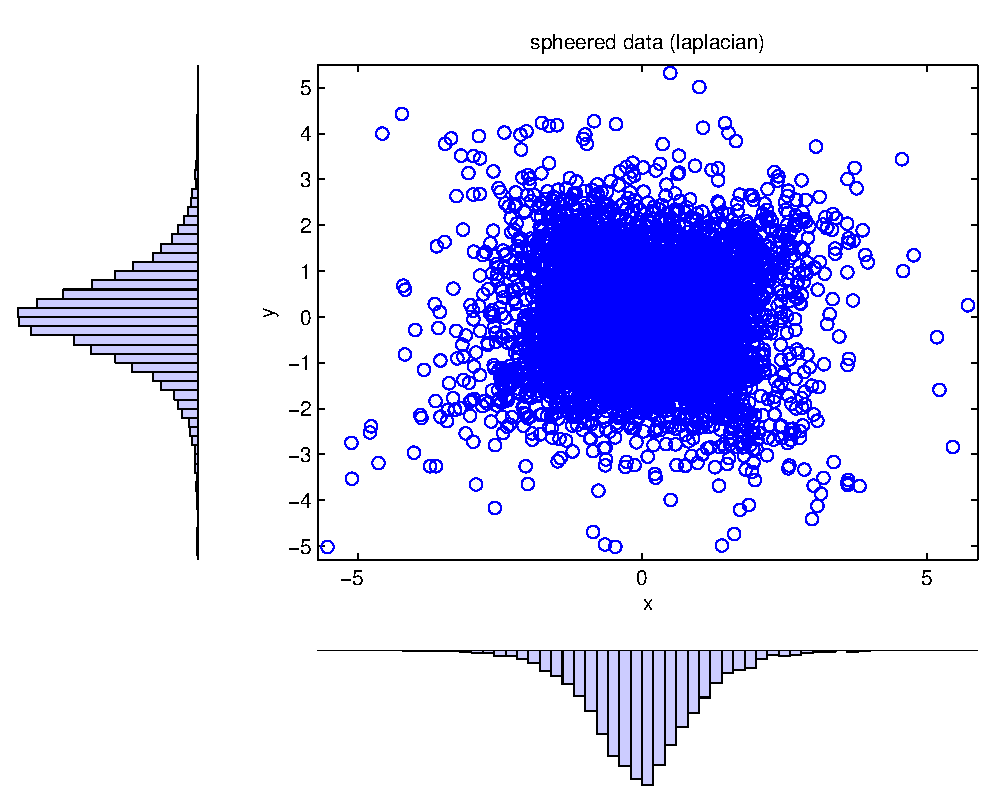
\includegraphics[scale = .4]{laplacian_spheered.eps}} 
\caption{Spheering laplacian distribution}
\end{figure}

\begin{figure}
\centering
\subfigure[kurtosis]{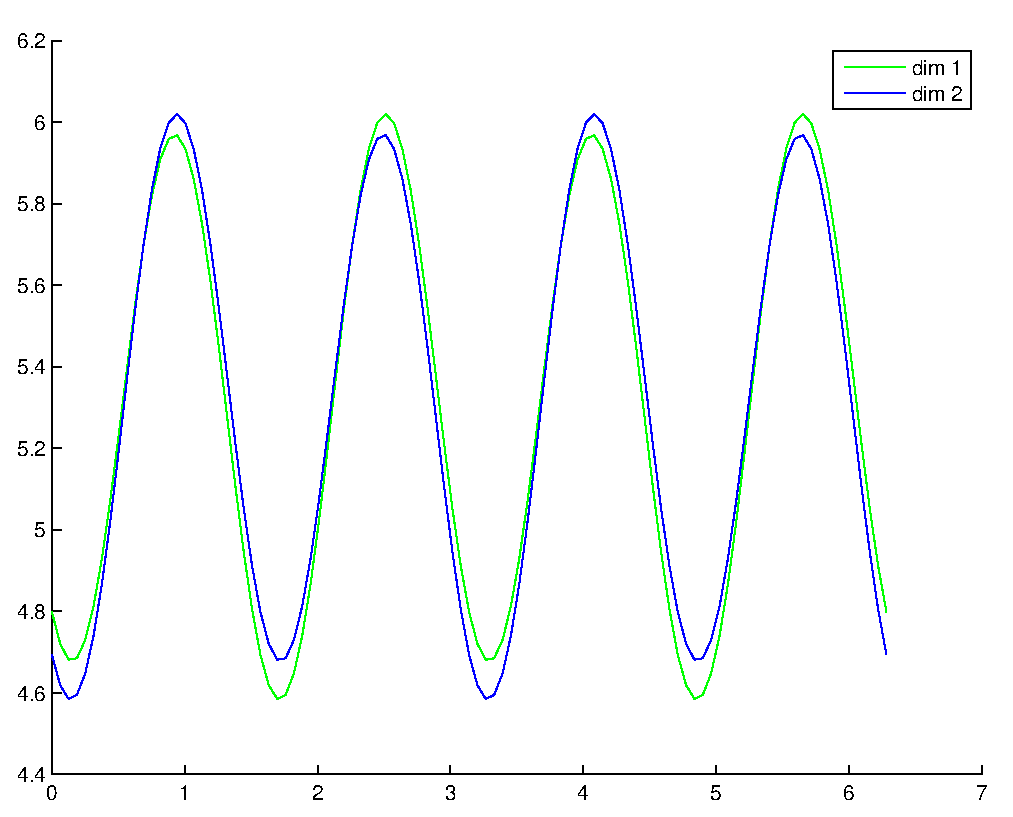
\includegraphics[scale = .4]{laplacian_kurtrot.eps}}\\
\subfigure[maximum kurtosis]{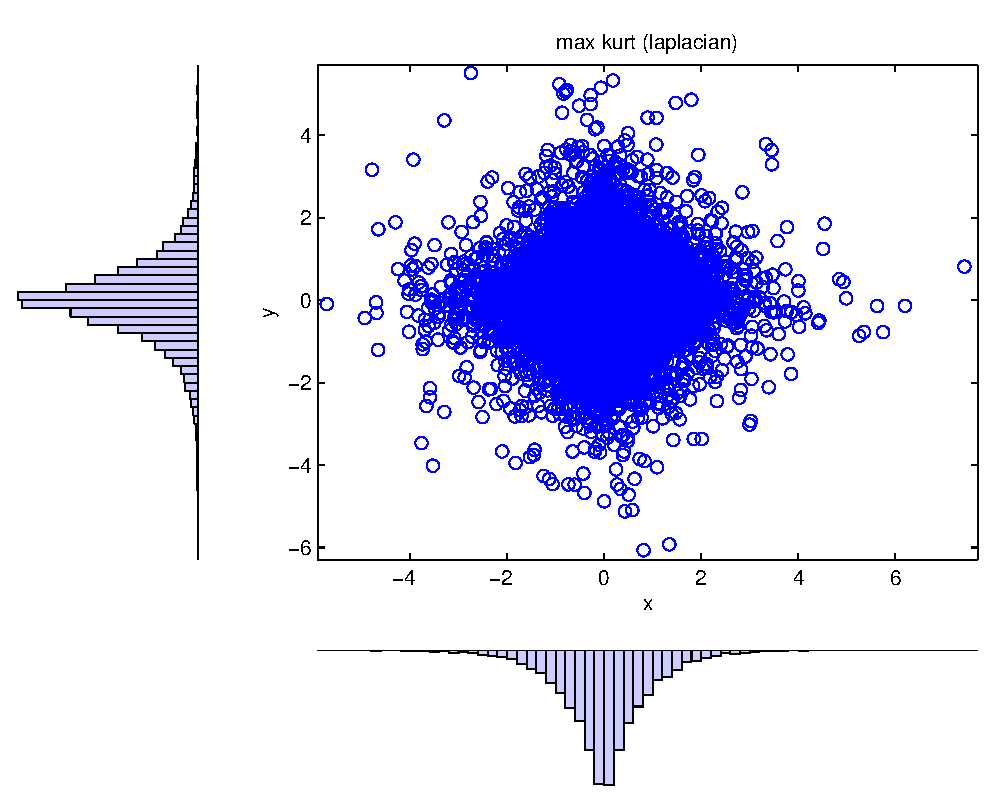
\includegraphics[scale = .4]{laplacian_maxkurt.eps}}\qquad
\subfigure[minimum kurtosis]{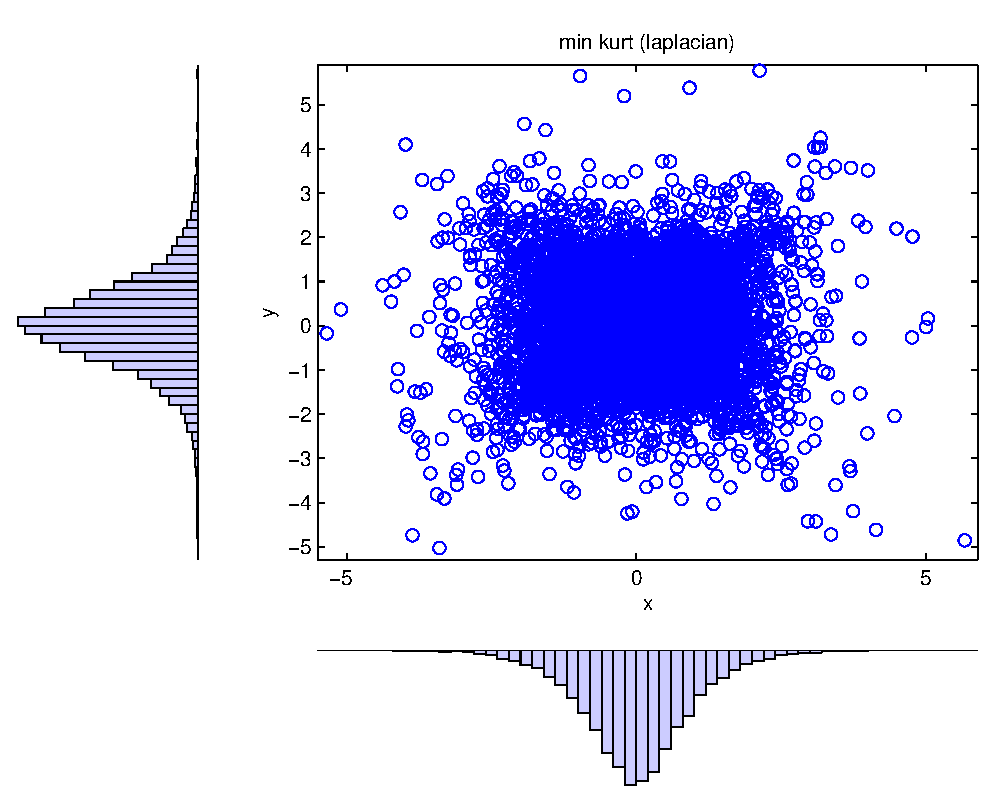
\includegraphics[scale = .4]{laplacian_minkurt.eps}} \\
\caption{Rotating laplacian distribution to find maximum and minimum kurtosis}
\end{figure}

\begin{figure}
\centering
\subfigure[original]{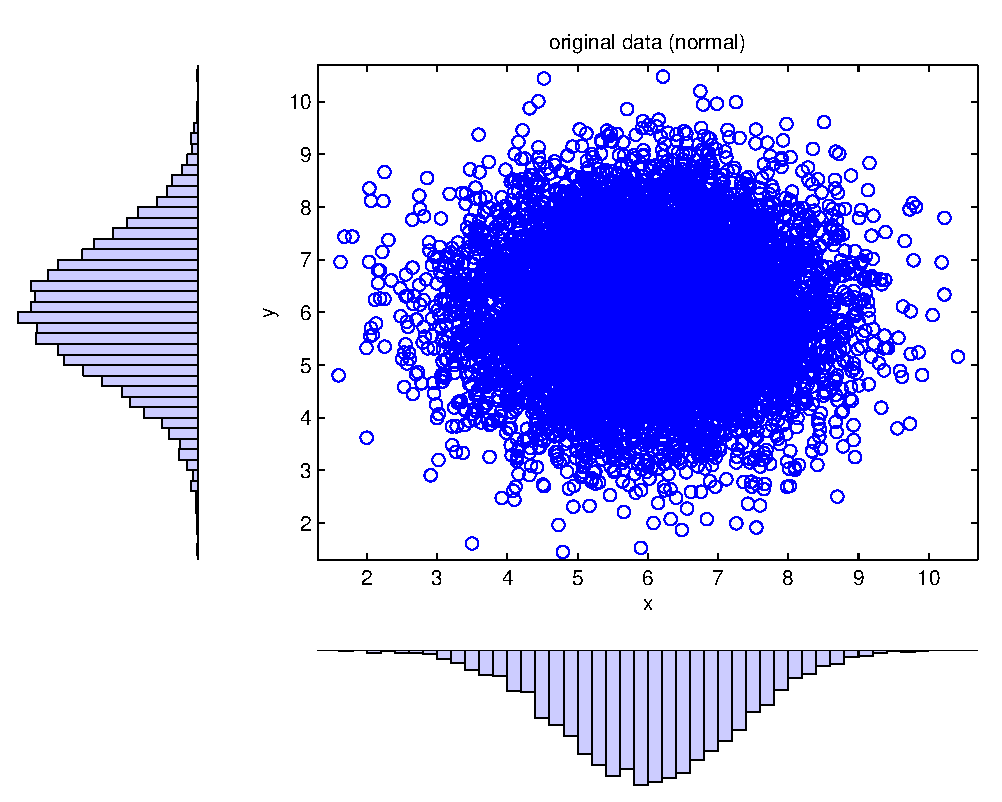
\includegraphics[scale = .4]{normal_original.eps}}\qquad
\subfigure[mixed]{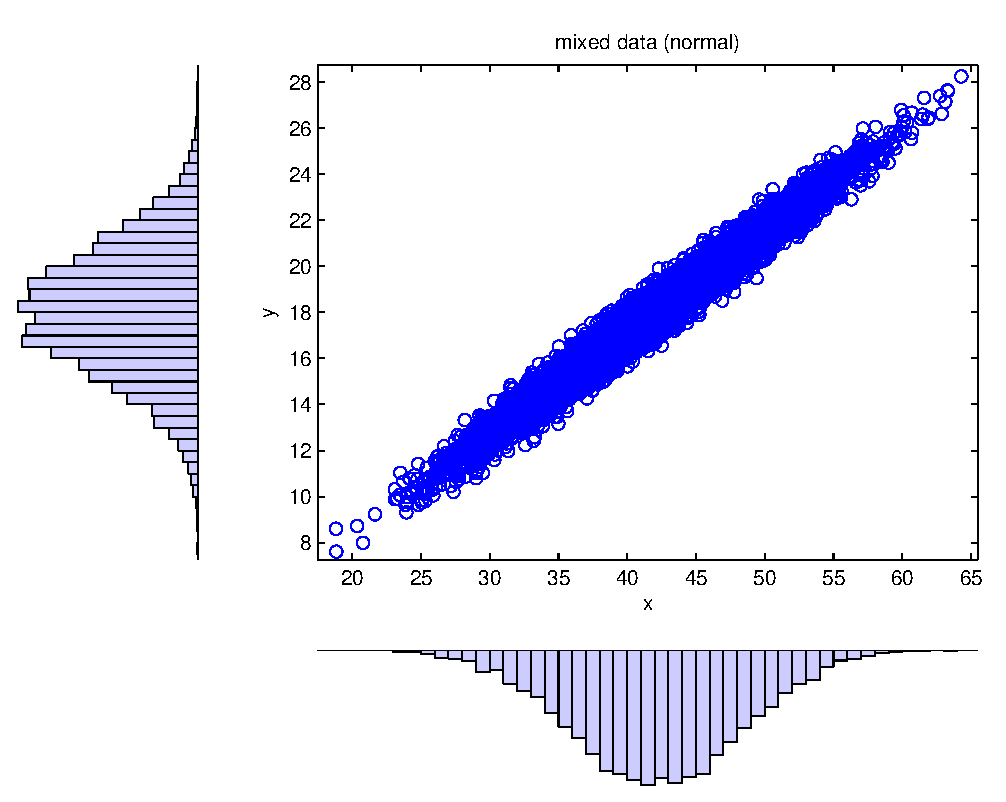
\includegraphics[scale = .4]{normal_mixed.eps}} \\
\subfigure[centered]{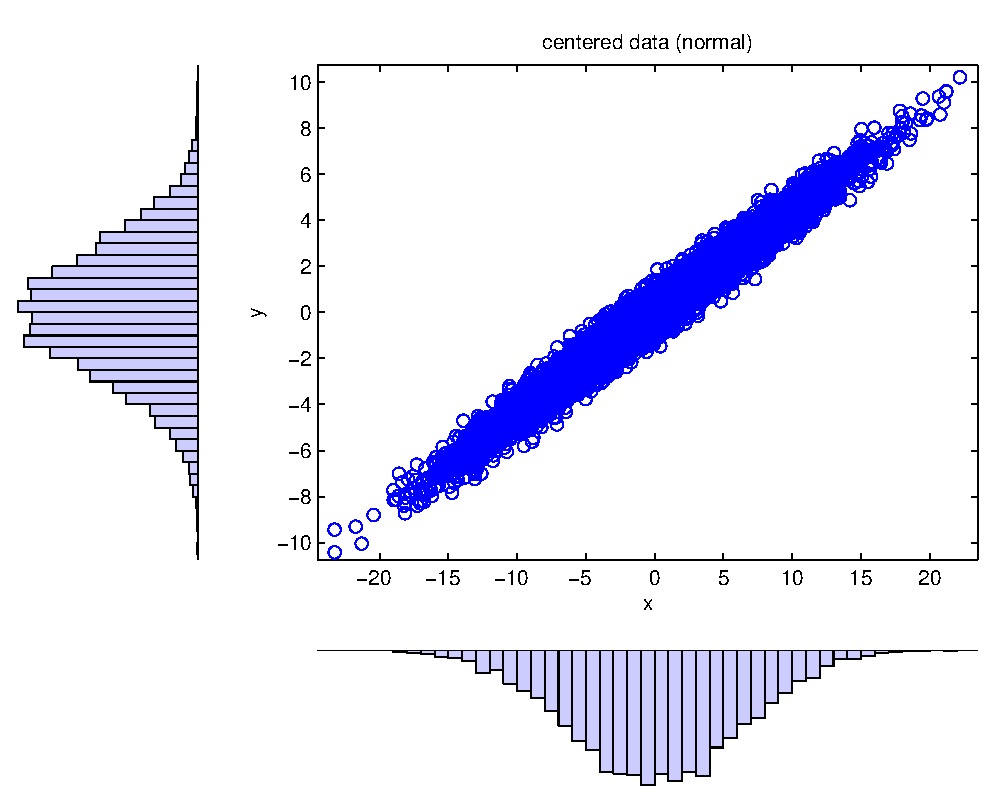
\includegraphics[scale = .4]{normal_centered.eps}}\qquad
\subfigure[decorellated]{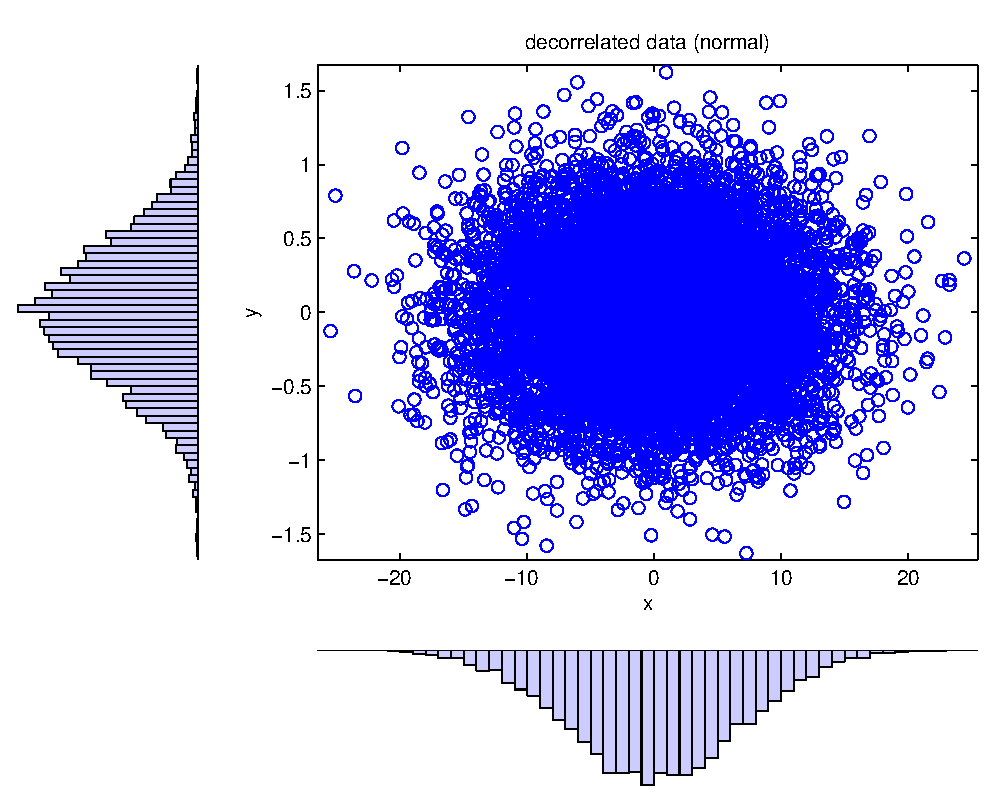
\includegraphics[scale = .4]{normal_decorellated.eps}} \\
\subfigure[spheered]{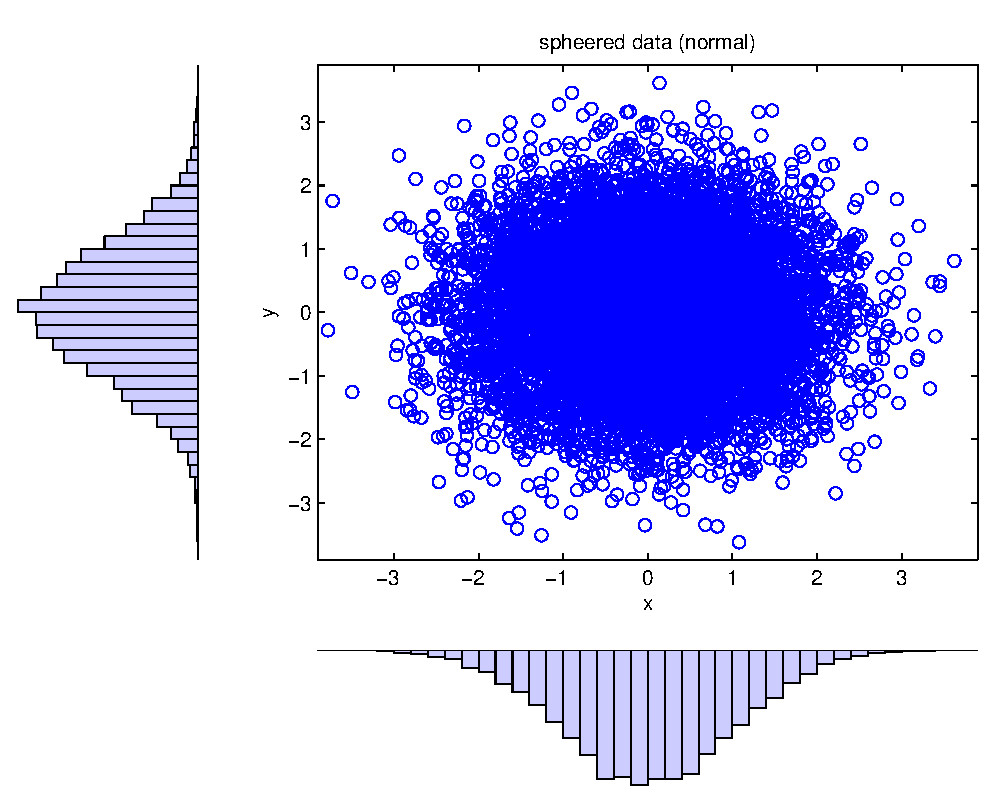
\includegraphics[scale = .4]{normal_spheered.eps}} 
\caption{Spheering normal distribution}
\end{figure}

\begin{figure}
\centering
\subfigure[kurtosis]{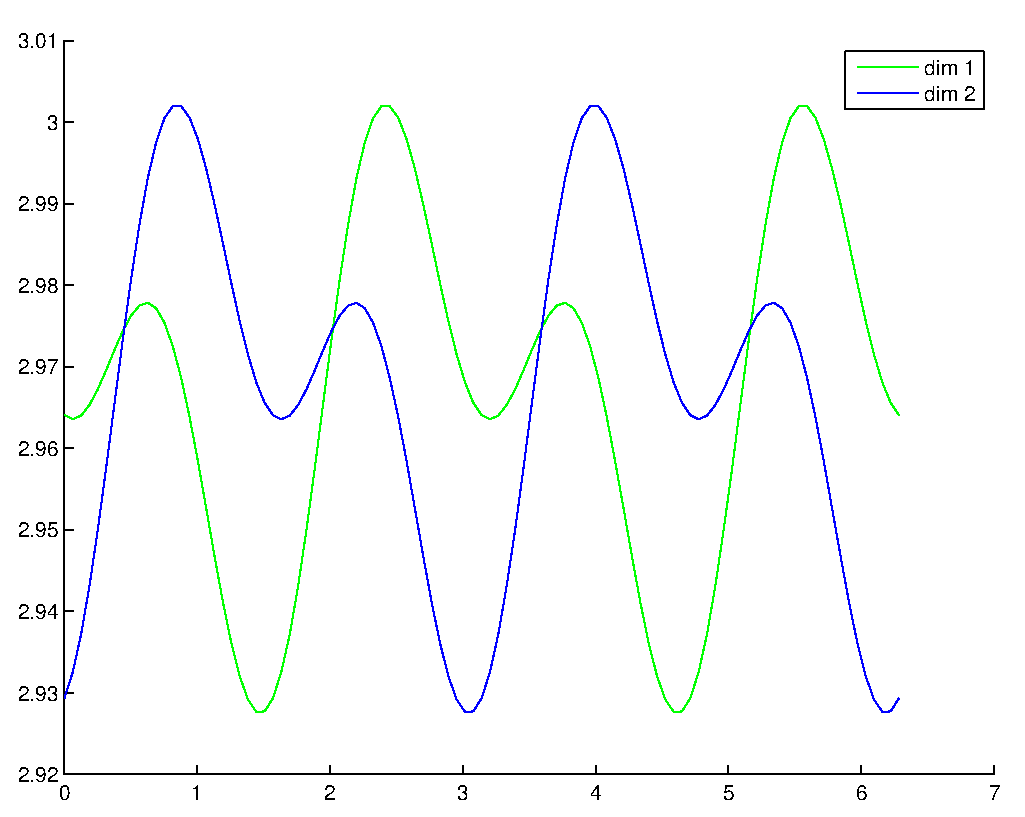
\includegraphics[scale = .4]{normal_kurtrot.eps}}\\
\subfigure[maximum kurtosis]{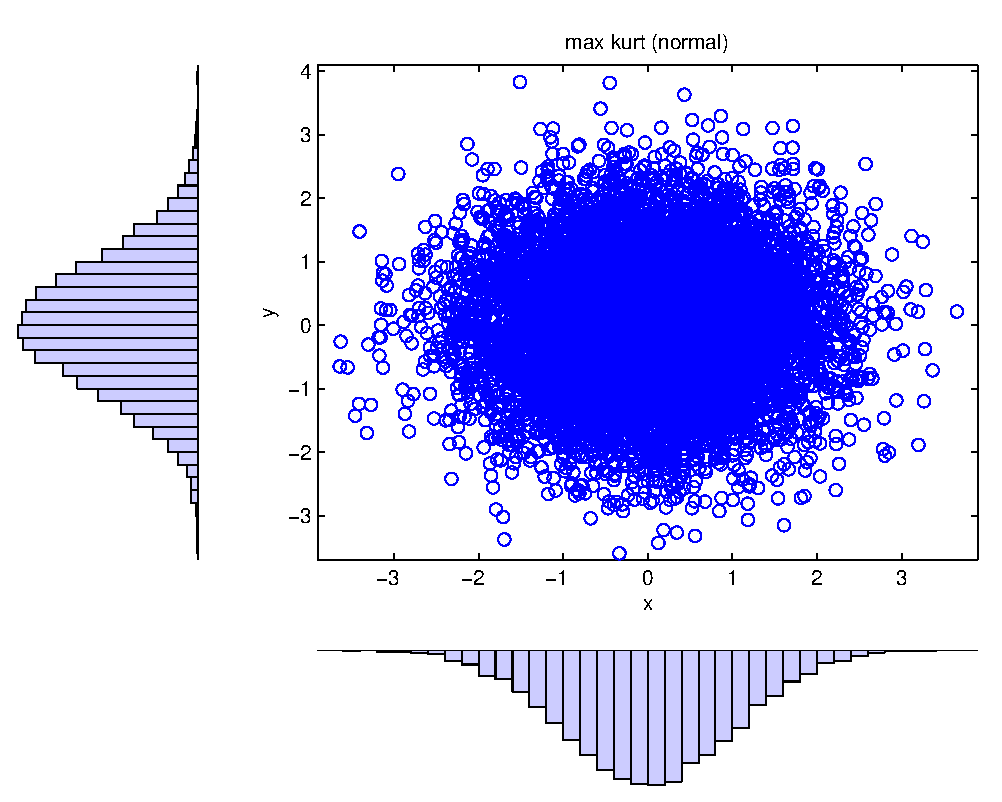
\includegraphics[scale = .4]{normal_maxkurt.eps}}\qquad
\subfigure[minimum kurtosis]{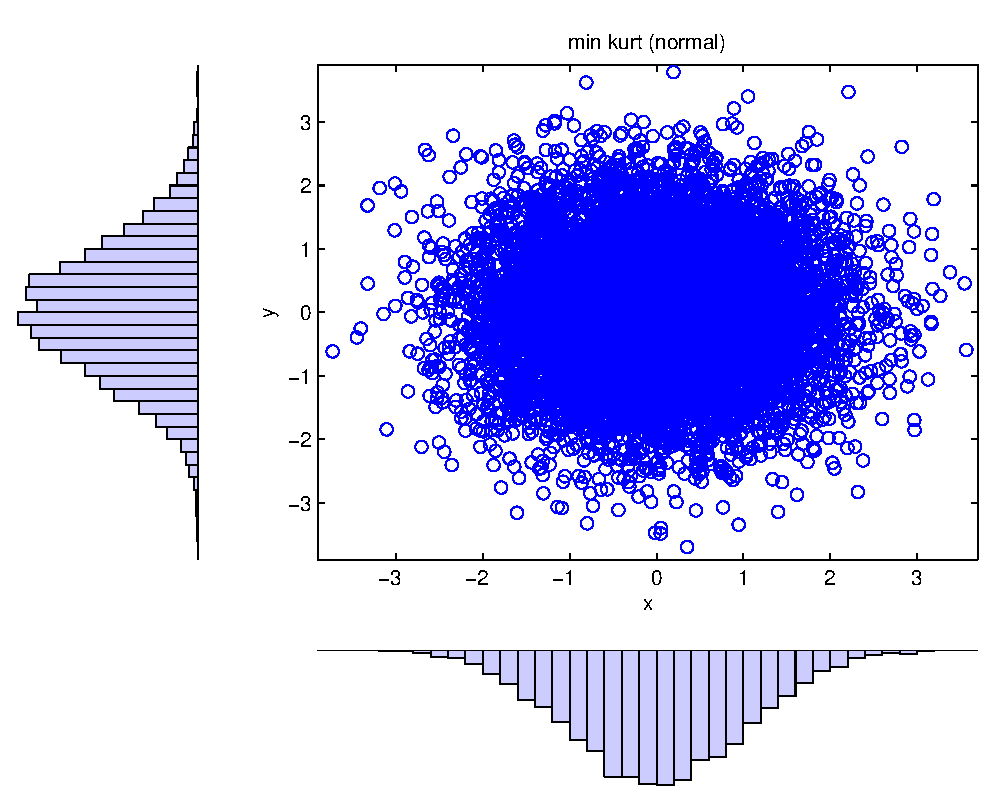
\includegraphics[scale = .4]{normal_minkurt.eps}} \\
\caption{Rotating normal distribution to find maximum and minimum kurtosis}
\end{figure}

\begin{figure}
\centering
\subfigure[original]{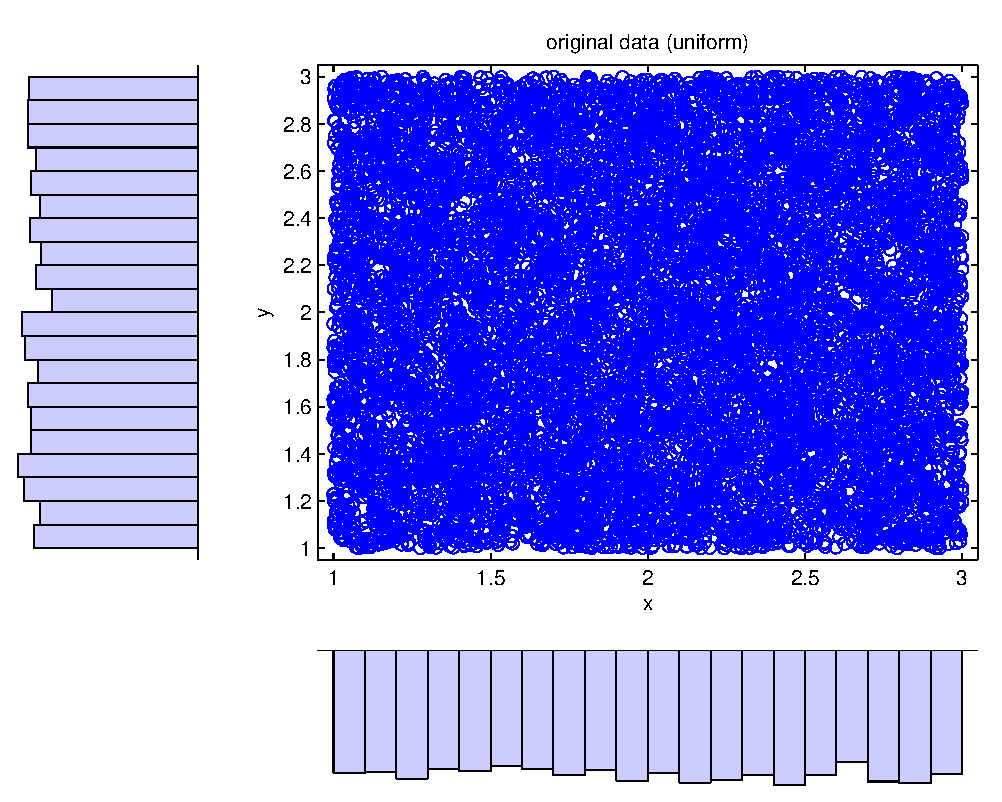
\includegraphics[scale = .4]{uniform_original.eps}}\qquad
\subfigure[mixed]{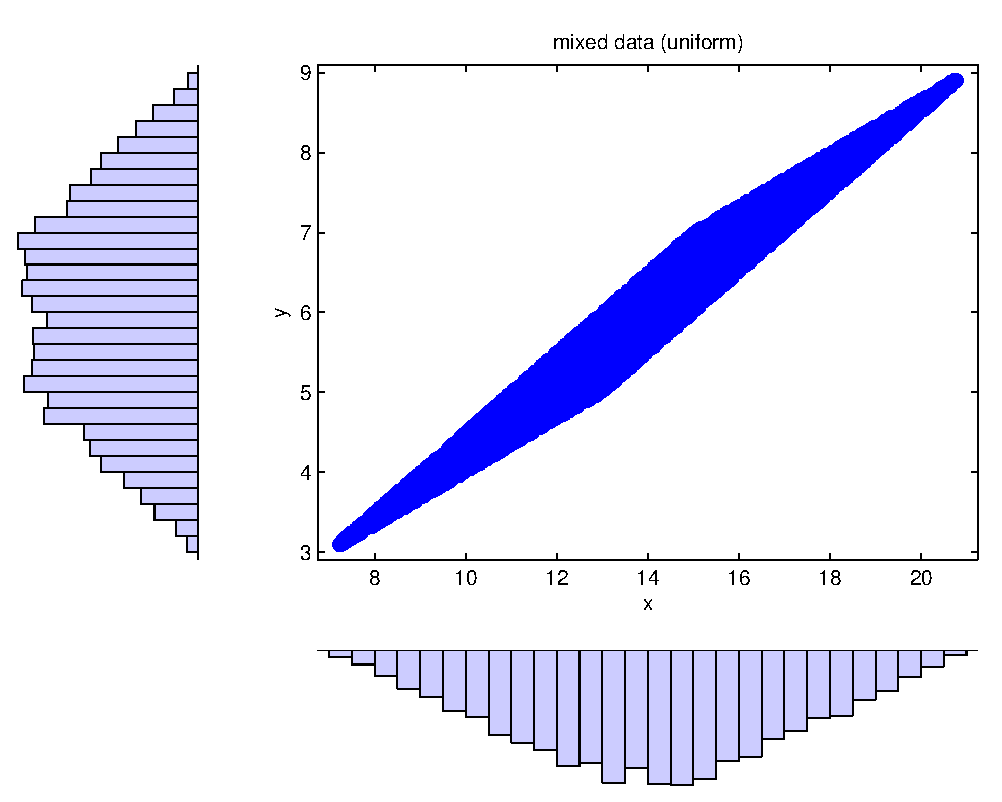
\includegraphics[scale = .4]{uniform_mixed.eps}} \\
\subfigure[centered]{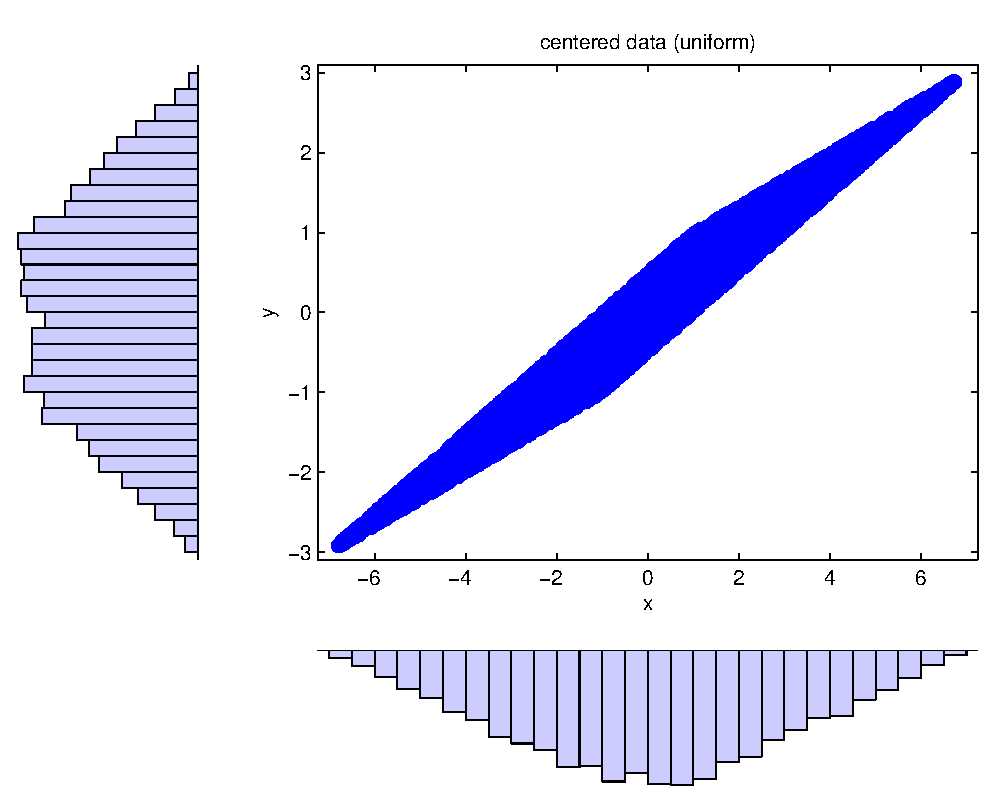
\includegraphics[scale = .4]{uniform_centered.eps}}\qquad
\subfigure[decorellated]{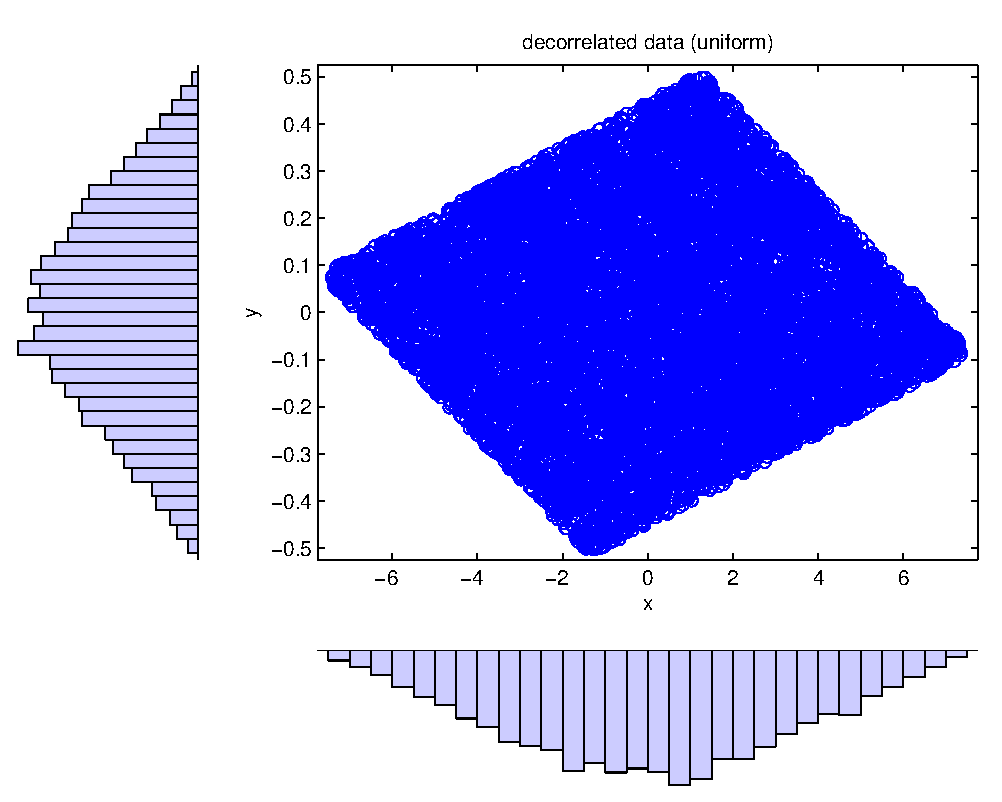
\includegraphics[scale = .4]{uniform_decorellated.eps}} \\
\subfigure[spheered]{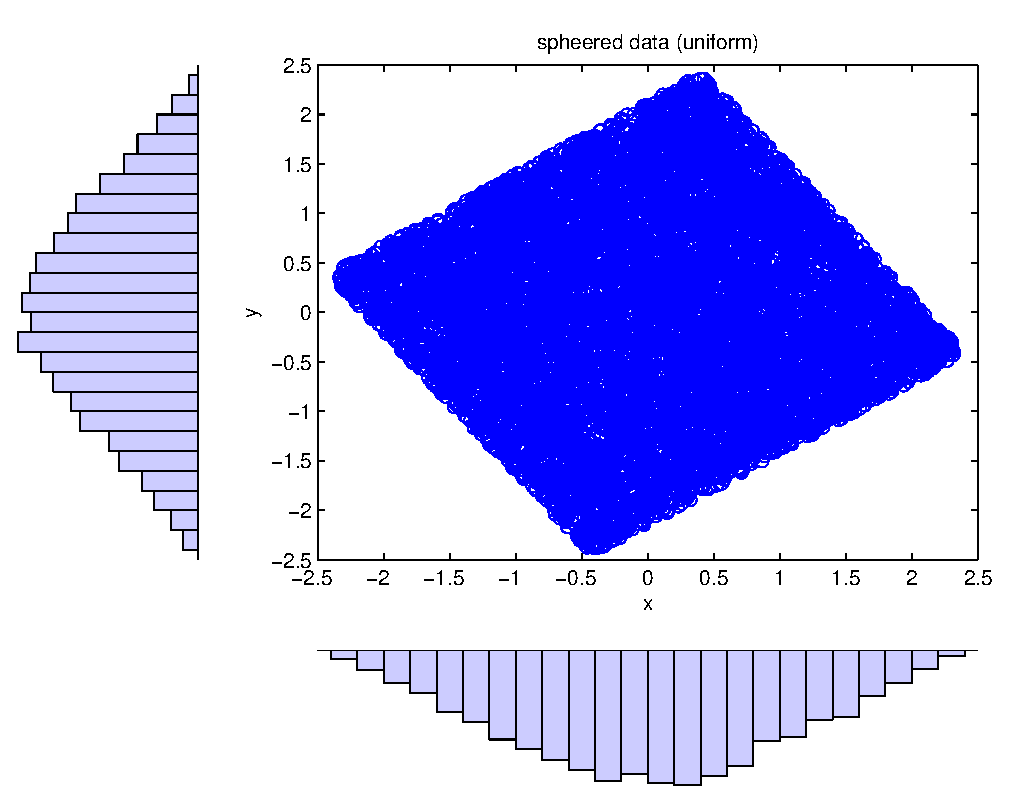
\includegraphics[scale = .4]{uniform_spheered.eps}} 
\caption{Spheering uniform distribution}
\end{figure}

\begin{figure}
\centering
\subfigure[kurtosis]{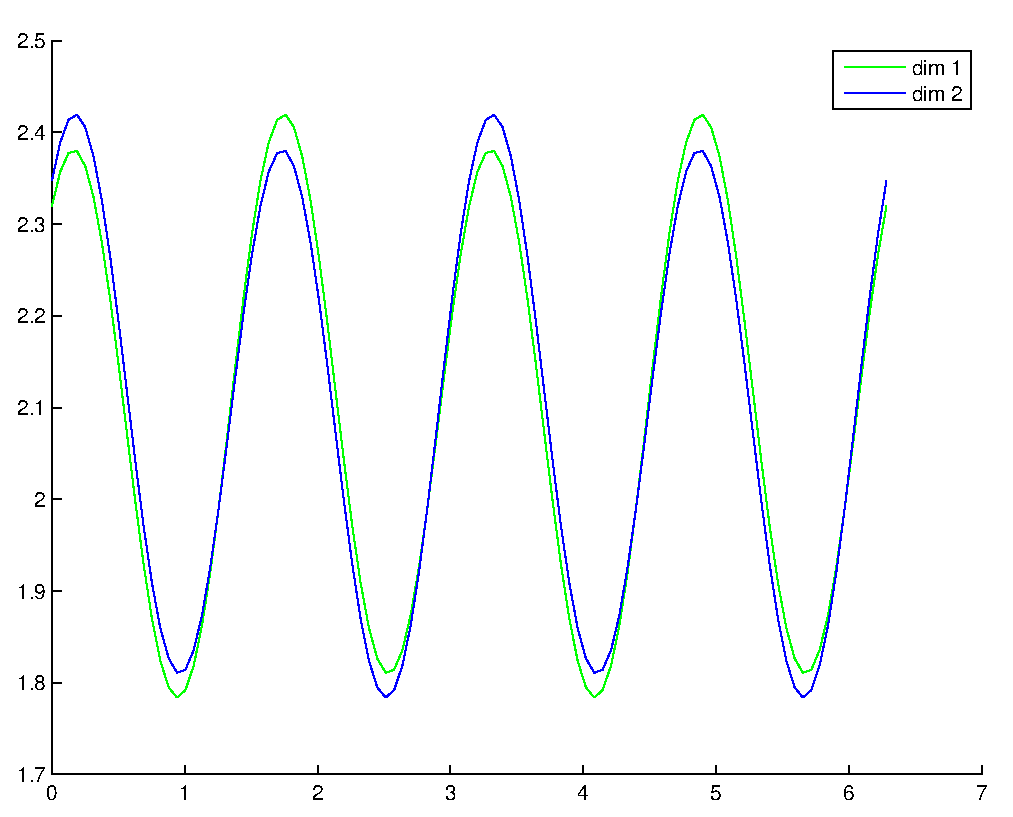
\includegraphics[scale = .4]{uniform_kurtrot.eps}}\\
\subfigure[maximum kurtosis]{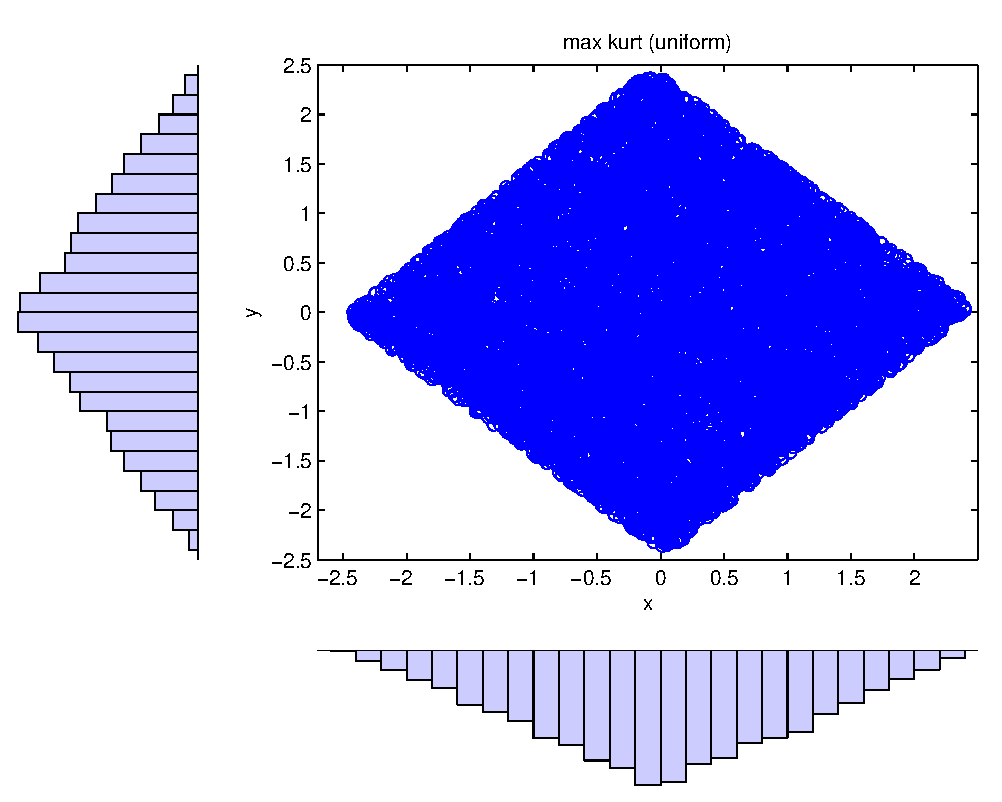
\includegraphics[scale = .4]{uniform_maxkurt.eps}}\qquad
\subfigure[minimum kurtosis]{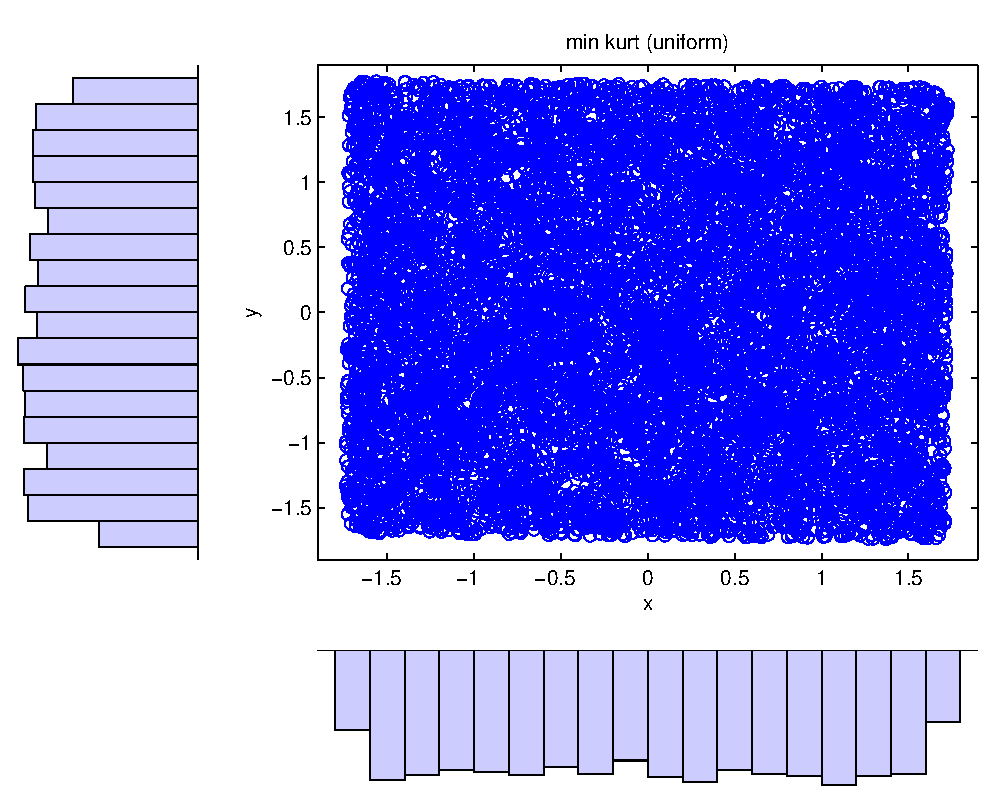
\includegraphics[scale = .4]{uniform_minkurt.eps}} \\
\caption{Rotating uniform distribution to find maximum and minimum kurtosis}
\end{figure}

\begin{figure}
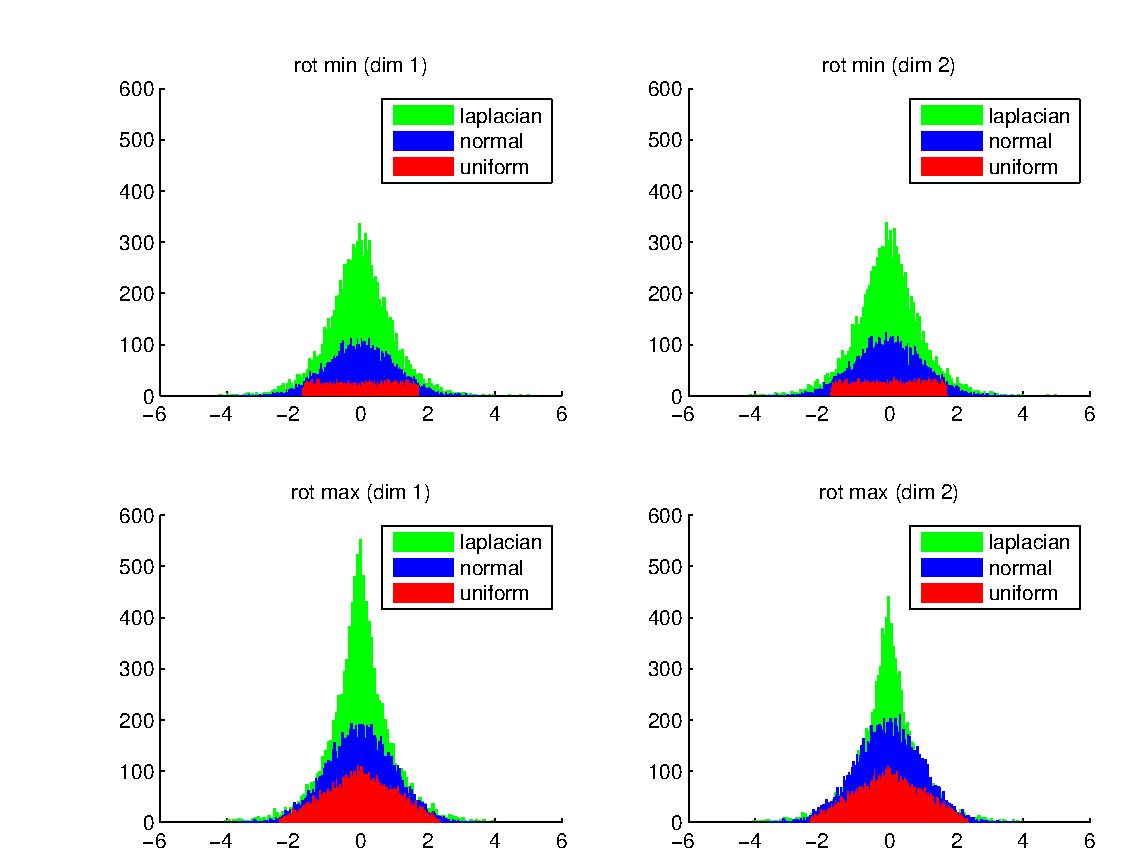
\includegraphics[scale = .8]{kurthist.eps}
\centering
\caption{Histogram comparison for maximum and minimum kurtosis}
\end{figure}

\clearpage

\section*{Exercise 2 - Toy Signal Separation}

In this exercise we mix three independent signals and we recover the original sources using the ICA algorithm.
All the sources have been recovered successfully, we also observe that sources can be recovered in different scales and different orders with respect to the original signals.

\begin{figure}[h!]
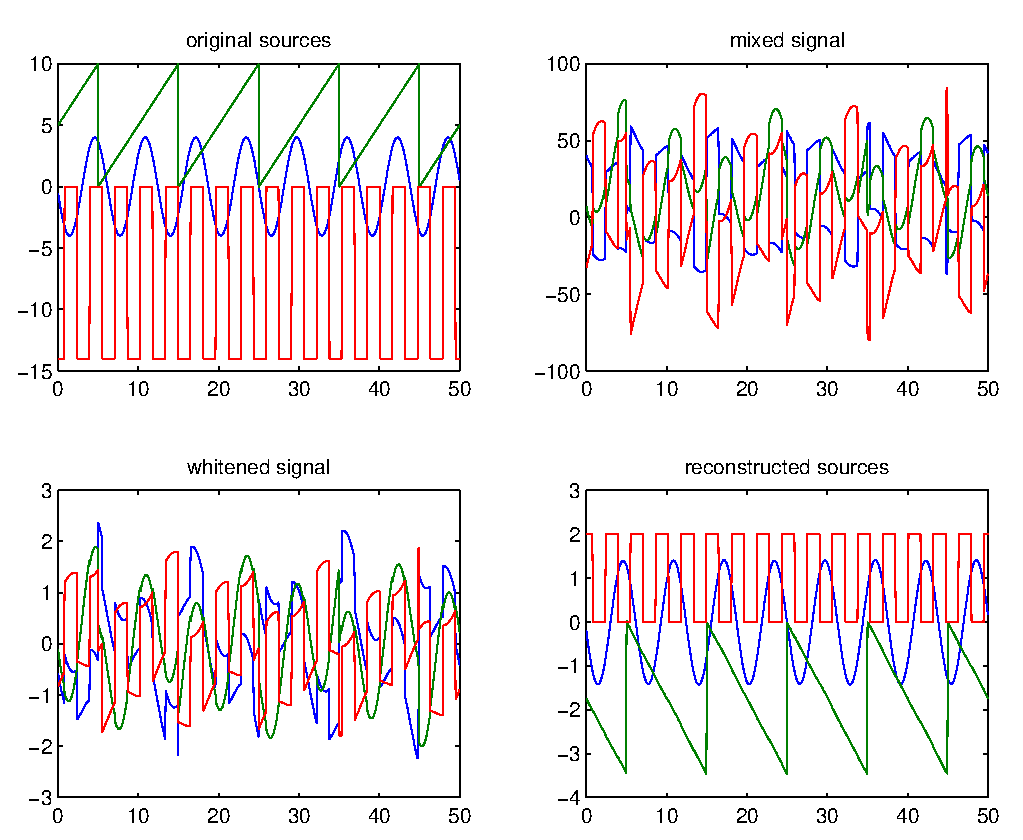
\includegraphics[scale = .8]{toysep.eps}
\centering
\caption{Toy signal separation}
\end{figure}

\clearpage

\section*{Exercise 3 - ICA on Image Patches}

In this exercise we apply ICA to image patches of different categories: nature, building and text.
We plot the columns of the mixing matrix $A$ estimated using the ICA algorithm. These represent distinctive independent features for each image category (only the first 20 independent features are shown). We can see that with natural images the independent features are gabor-like functions and resemble the natural basis of the Fourier domain. 
As expected, for images of buildings we observe more edgy features while for the text category we obtain both edgy and gabor-like independent features.

\begin{figure}[h!]
\centering
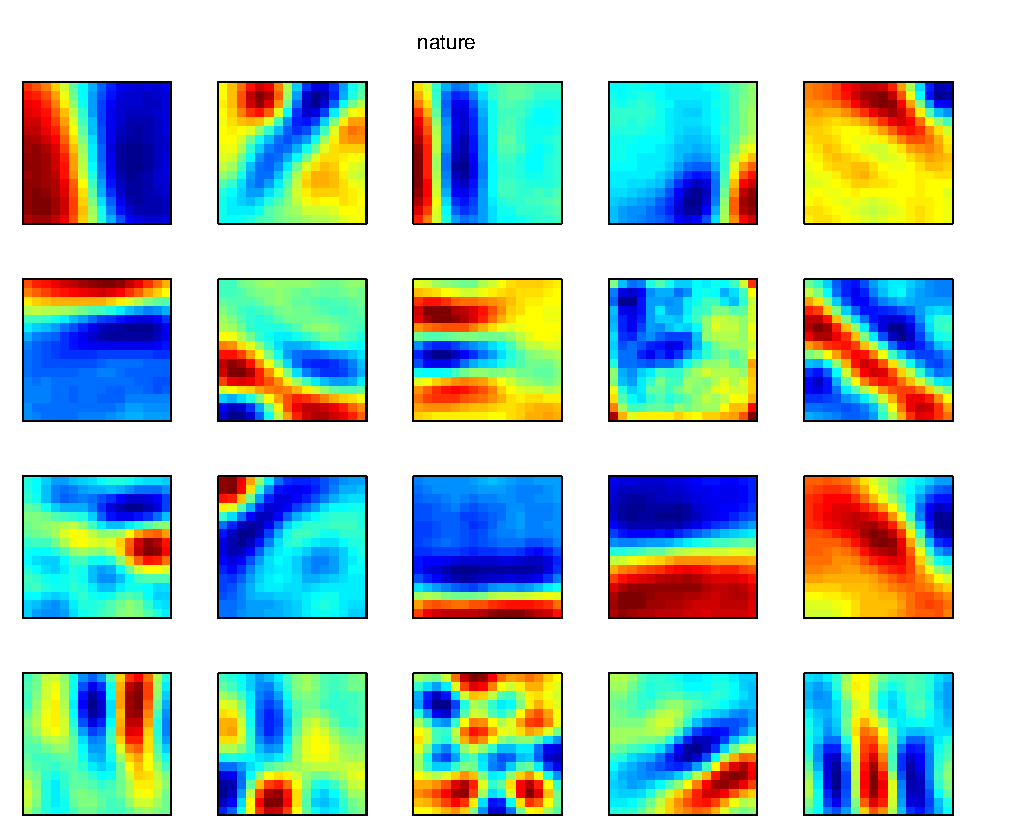
\includegraphics[scale = .7]{nature_indfeats.eps}
\caption{First 20 independent features extracted from \emph{nature} image patches}
\end{figure}

\begin{figure}[h!]
\centering
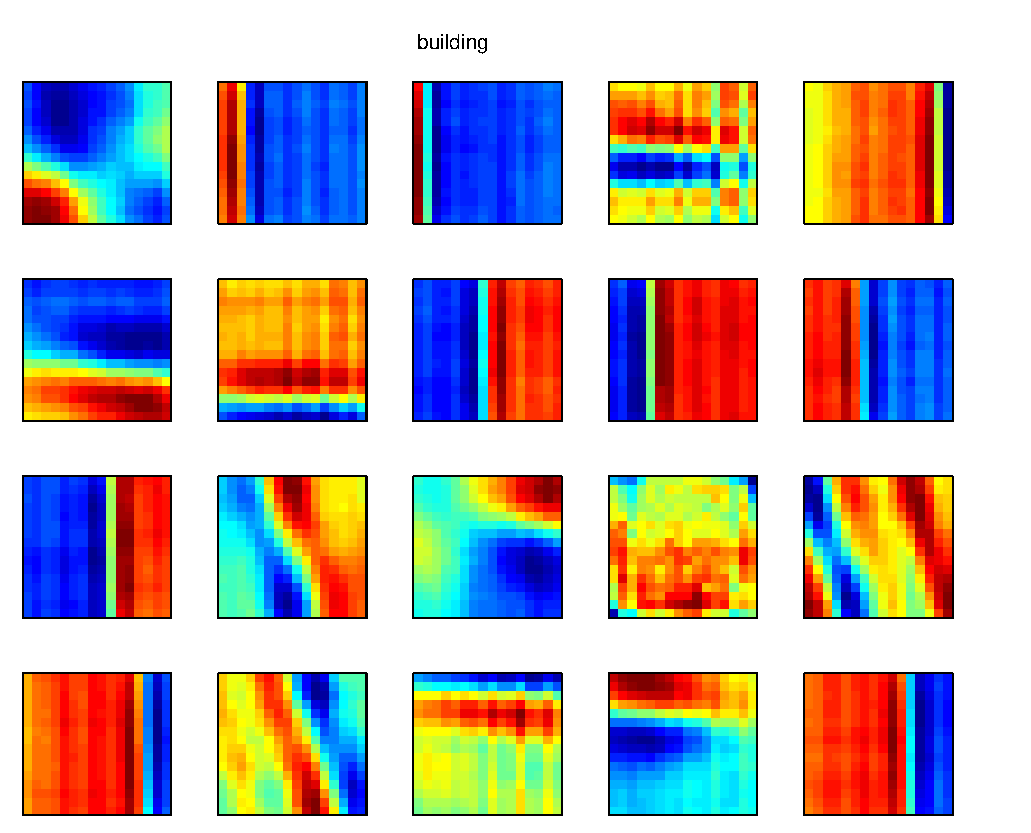
\includegraphics[scale = .7]{building_indfeats.eps}
\caption{First 20 independent features extracted from \emph{building} image patches}
\end{figure}

\begin{figure}[h!]
\centering
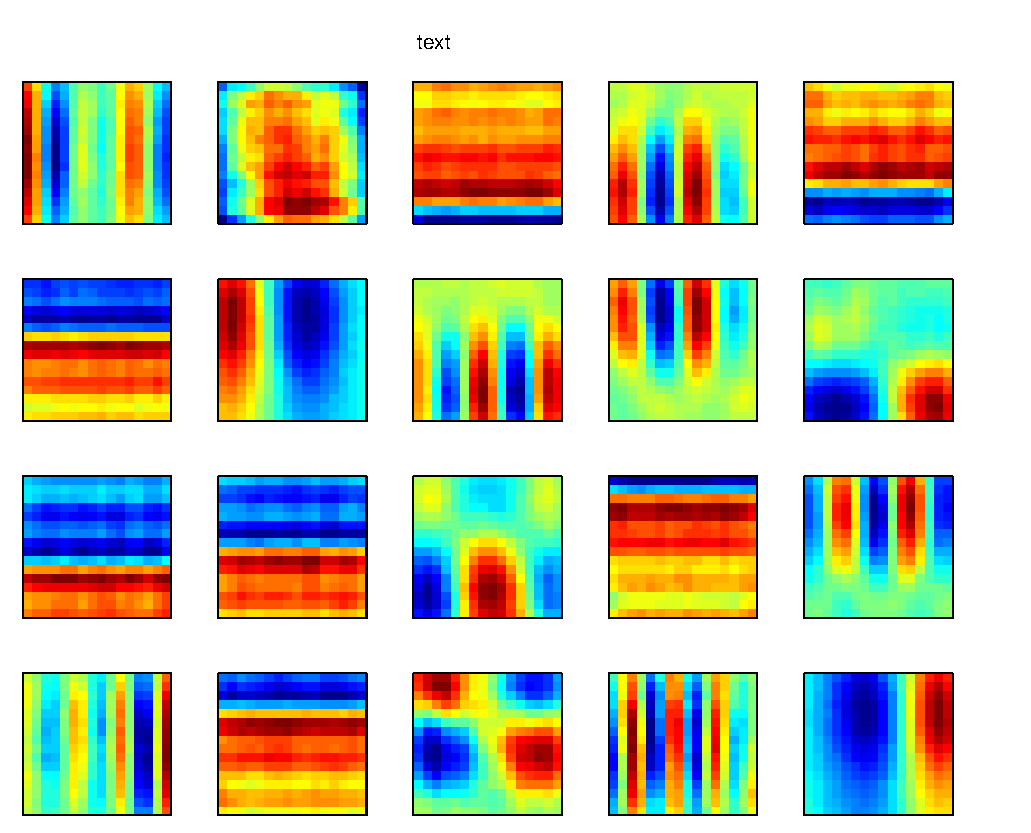
\includegraphics[scale = .7]{text_indfeats.eps}
\caption{First 20 independent features extracted from \emph{text} image patches}
\end{figure}
\end{document}
